\documentclass[tikz,border=4pt]{standalone}
\usepackage{ctex}
\usepackage{pgfplots}
\pgfplotsset{compat=1.18}
\begin{document}
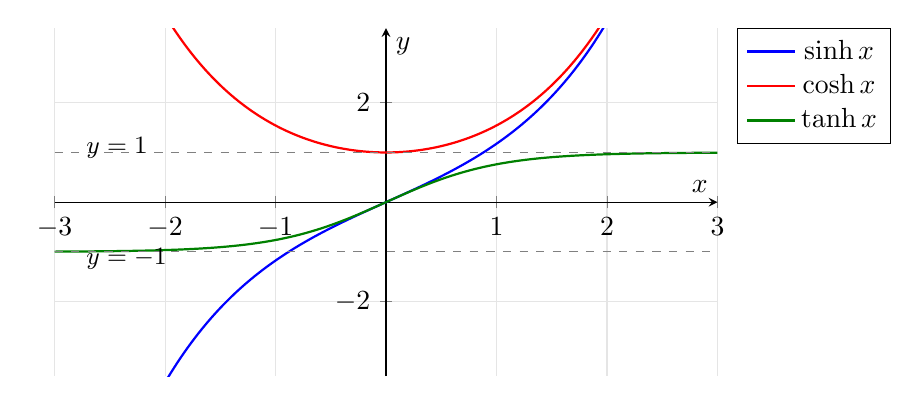
\begin{tikzpicture}
\begin{axis}[
    axis lines=middle, width=10cm, height=6cm,
    xmin=-3, xmax=3, ymin=-3.5, ymax=3.5,
    samples=200, grid=both, grid style={gray!20},
    xlabel={$x$}, ylabel={$y$},
    legend pos=outer north east,
]
\addplot[blue, thick, domain=-3:3] {sinh(x)};
\addlegendentry{$\sinh x$}
\addplot[red, thick, domain=-3:3] {cosh(x)};
\addlegendentry{$\cosh x$}
\addplot[green!50!black, thick, domain=-3:3] {tanh(x)};
\addlegendentry{$\tanh x$}
\draw[gray, dashed] (axis cs:-3,1) -- (axis cs:3,1);
\draw[gray, dashed] (axis cs:-3,-1) -- (axis cs:3,-1);
\node[anchor=west] at (axis cs:-2.8,1.1) {\small $y=1$};
\node[anchor=west] at (axis cs:-2.8,-1.15) {\small $y=-1$};
\end{axis}
\end{tikzpicture}
\end{document}
